\section{Data Acquisition}

\subsection{Experimental Setup}
The data acquisition was performed with four LiDARs, namely the SICK LMS200, the SICK LMS151, the Hokuyo UTM-30LX-EW and the Velodyne HDL-32E. A camera was also used to get visual information about the scene. Table~\ref{tab:lidars} gives additional informations about the LiDARs. Note that all LiDARs use class 1 laser with a wavelength of \SI{905}{\nano\meter}.
~\cite{VelodyneManual}
~\cite{UTMDatasheet}
~\cite{LMS151Datasheet}
~\cite{LMS200Manual}

\begin{table}[htbp]
    \centering
    \begin{tabularx}{\linewidth}{|X|X|X|X|X|}\hline
        \textbf{Sensor}             & \textbf{Echoes}  & \textbf{Maximum Distance}\footnote{The maximum distance depends on several factors such as lighting conditions and target remission. SICK distances are given for target remission greater than 75\%.}  & \textbf{Spot Area (at 30 meters)} & \textbf{Spot Shape}  \\ \hline
        SICK LMS200        & 1       & \SI{28}{\meter}   & \SI{165}{\centi\meter\squared}     & Circle     \\ \hline
        SICK LMS151        & 2\footnote{Two echoes are evaluated by the sensor, but only one is returned}       & \SI{50}{\meter}   & \SI{22}{\centi\meter\squared}      & Circle     \\ \hline
        Hokuyo UTM-30LX-EW & 3       & \SI{30}{\meter}   & \SI{196}{\centi\meter\squared}     & Ellipse    \\ \hline
        Velodyne HDL-32E   & 1       & \SI{70}{\meter}   & \SI{51}{\centi\meter\squared}      & Rectangle  \\ \hline
    \end{tabularx}
    \caption{LiDARs information}\label{tab:lidars}
\end{table}

The sensors were placed close to the inner wall of a window facing N\SI{50}{\degree}E. A wooden structure held the LiDARs side by side at approximately \SI{13.9}{\meter} above the ground and the main scanning plane (i.e. \SI{0}{\degree} in the sensor reference frame) forming a \SI{30}{\degree} angle with respect to the building wall. In this configuration, a slight opening of the window allowed to keep the LiDARs inside while scanning outside. To avoid direct light exposure between sensors, corrugated plastic layers were placed between them. Note that we observed no interference between the sensor readings. Figure~\ref{fig:setup} present an overview of the setup.

\begin{figure}[h]
    \centering
    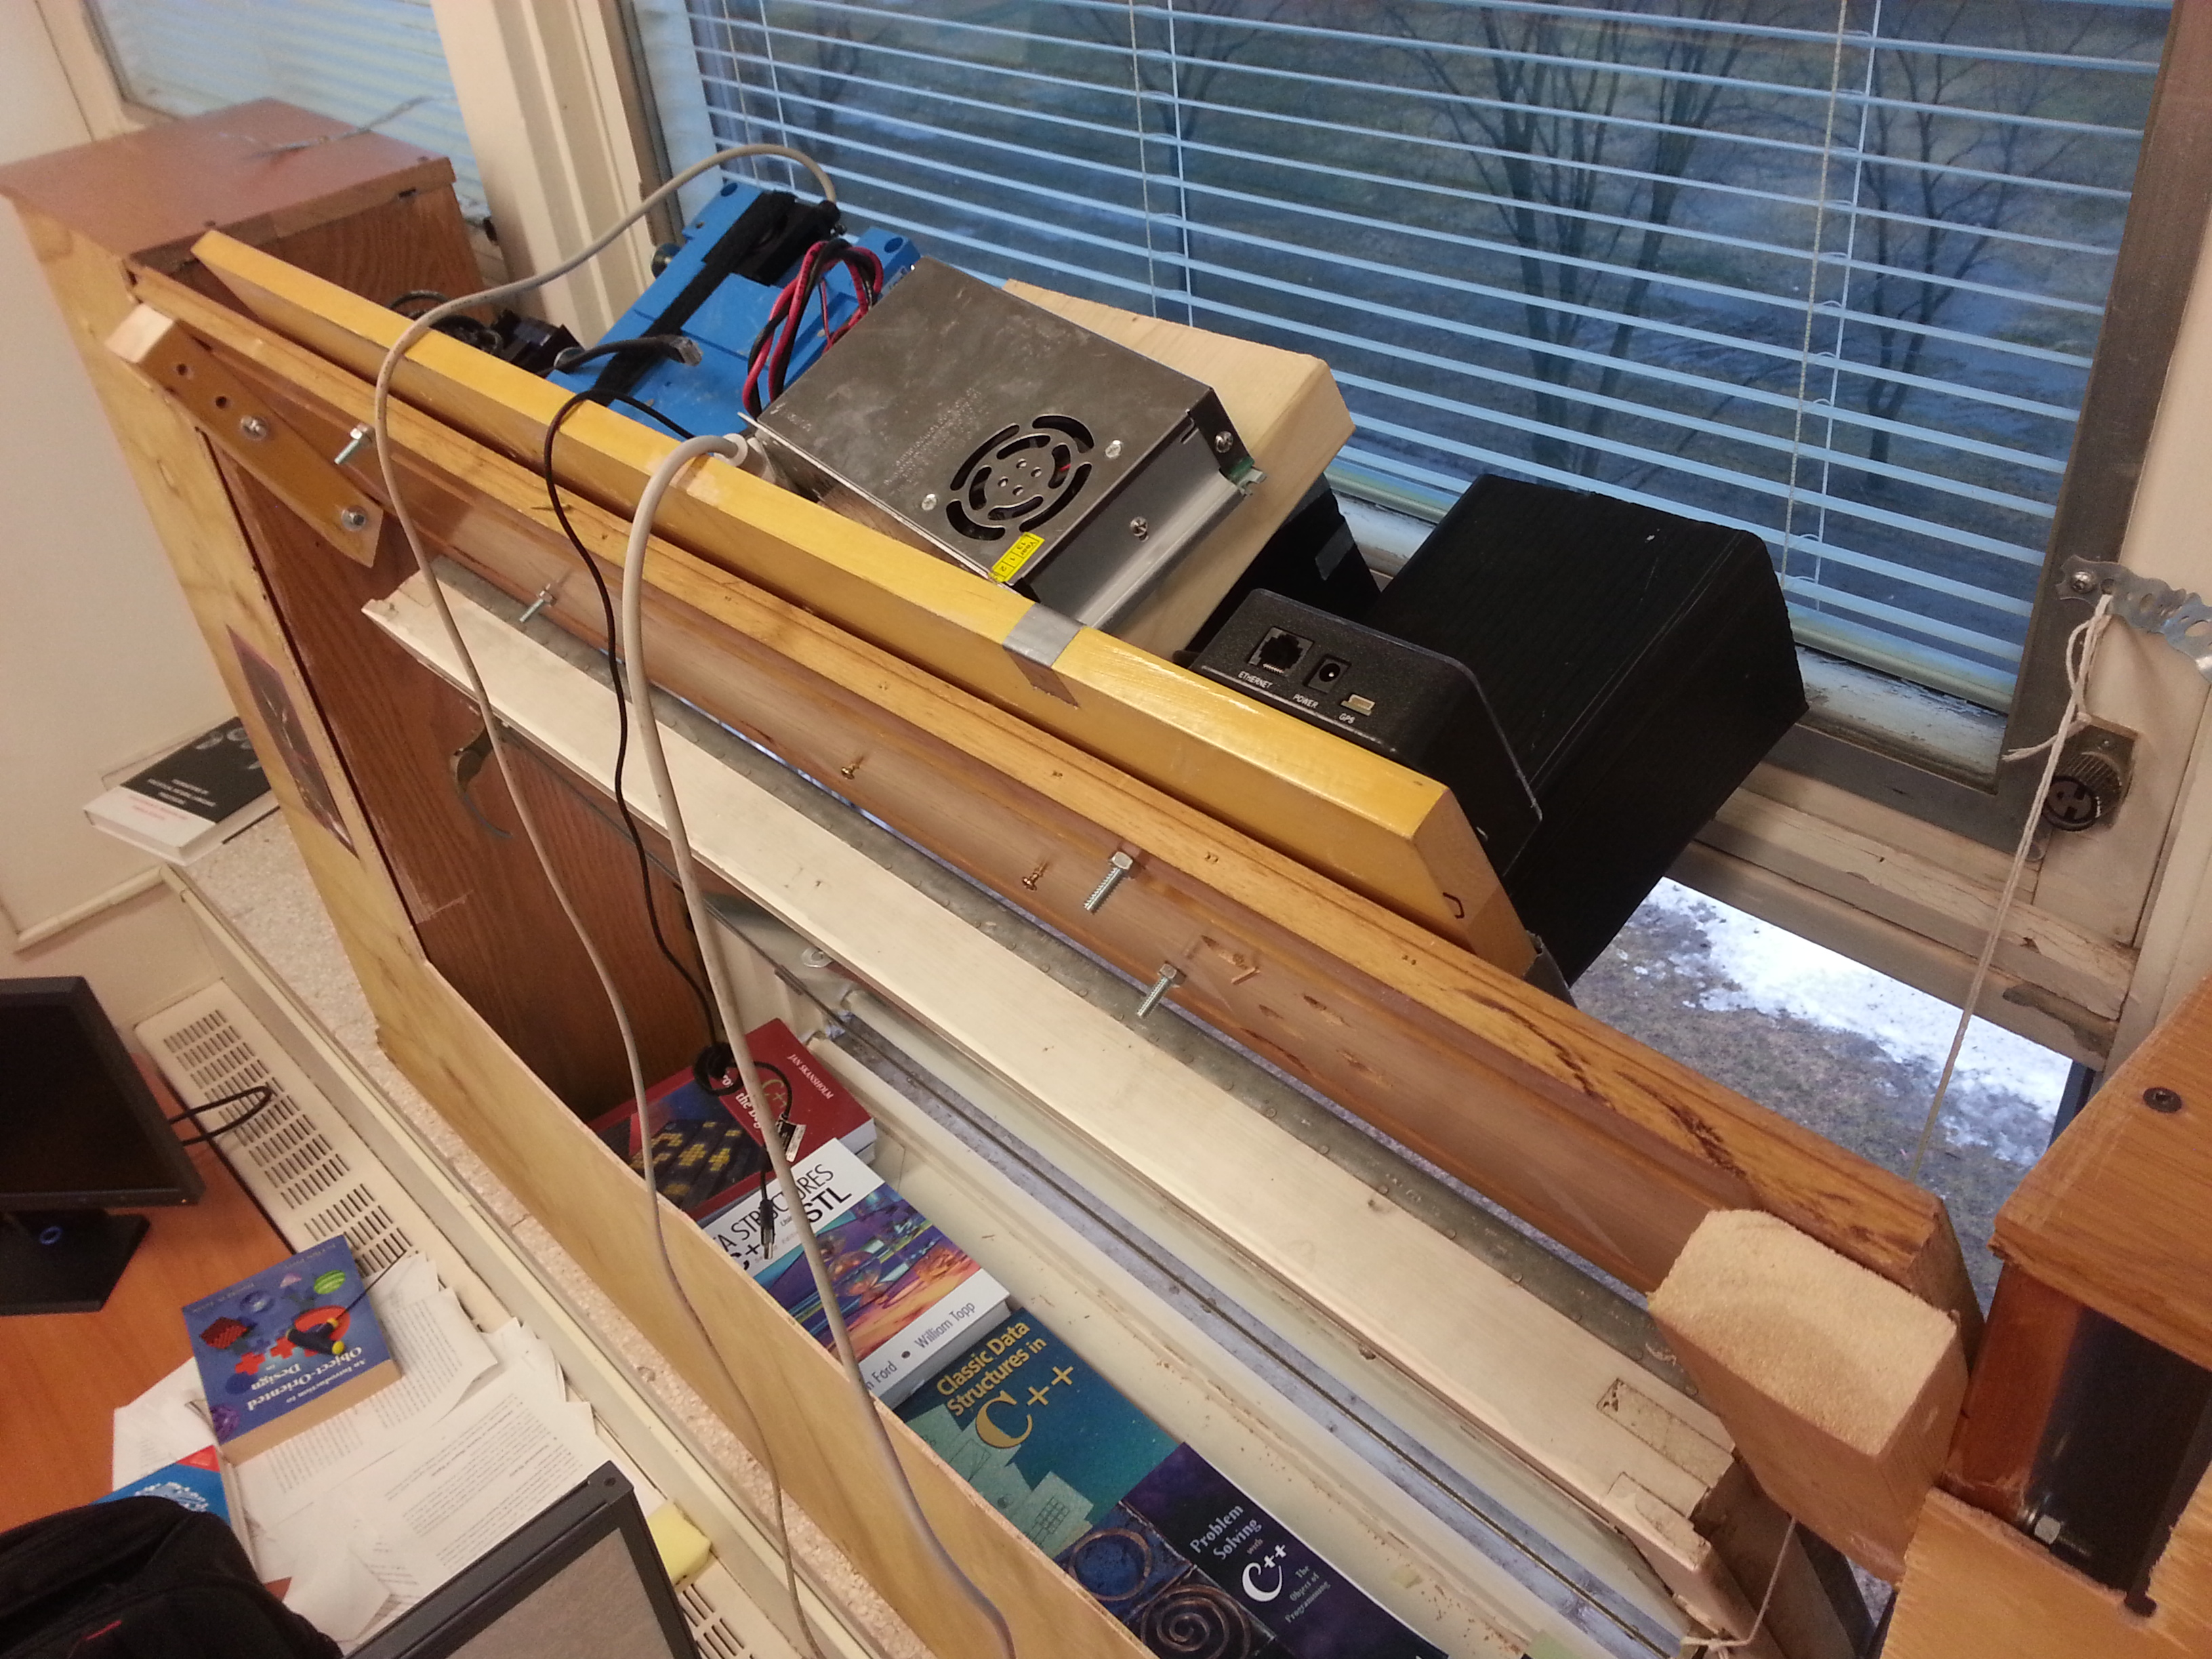
\includegraphics[width=0.95\linewidth]{./img/setup_diag.png}
    \caption{The experimental setup. The 3D axis represent the orientation of the sensors and the bottom left panel represent the 2D geometry as seen from the right side of the picture.}
    \label{fig:setup}
\end{figure}

The orientation of the building relative to the sun cause a shadow on the ground where the... The ground was not completely flat and even.

\subsection{Dataset Description}
Describe the overall data (table that is in the google drive) in this section... Over a wide variety of temperature, cloudy not cloudy, different size of flakes windy...

Data acquisition was conducted at Pouliot Pavilion of Laval University beginning February~11 and ending March~21.

% TODO remove the useless info about packages and messages
Recording of data was made through the Hydro distribution of the Robot Operating System (ROS)~\cite{ROSWeb}, which provide standardized data type as well as time synchronisation. The sicktoolbox\_wrapper~\cite{LMS200Web}, lms1xx~\cite{LMS151Web} and urg\_node~\cite{HokuyoWeb} packages provided \textit{LaserScan messages}\footnote{The LaserScan message definition is available at http://docs.ros.org/api/sensor\_msgs/html/msg/LaserScan.html} for the LMS200, LMS151 and UTM-30LX-EW respectively. The velodyne package~\cite{VelodyneWeb} produced the \textit{PointCloud2 messages}\footnote{The PointCloud2 message definition is available at http://docs.ros.org/api/sensor\_msgs/html/msg/PointCloud2.html} for the HDL-32E.

\begin{figure}[h]
    \centering
    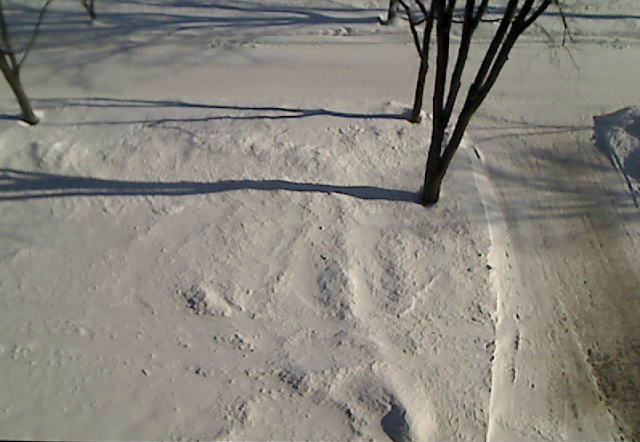
\includegraphics[width=0.90\linewidth]{./img/camera_view.jpg}
    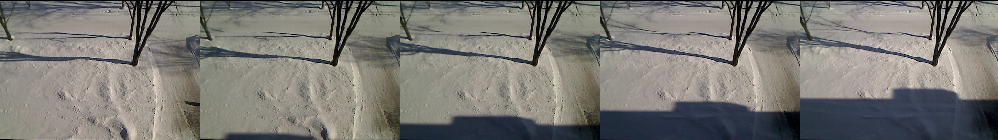
\includegraphics[width=0.95\linewidth]{./img/shadow2.png}
    \caption{View from the RGB camera. The sequence of pictures at the bottom shows the evolution of the shadow caused by the building between 10:00~am and 10:40~am.}
    \label{fig:setup}
\end{figure}

%Some notes to fill up the table:
%\begin{itemize}
    %\item LMS200
        %\begin{itemize}
            %\item See page 8. Range vs reflectivity
            %\item See page 7. It is around 20cm at 20m
        %\end{itemize}
    %\item LMS151
        %\begin{itemize}
            %\item See page 25. Scanning range up to 50 m (164.04 ft) with $>$ 75\% object remission (18 m (59.06 ft) with 10\% object remission)
            %\item See page 26. $distance(mm (in)) * 0.015 rad + 8 mm (0.31 in)$
        %\end{itemize}
    %\item Hokuyo
        %\begin{itemize}
            %\item 0.1 to 10m : $\pm$30mm,10 to 30m : $\pm$50mm(White Kent Sheet)
            %\item See article : Spot size is 50 mm × 500 mm at sensor’s maximum distance of 30 m
            %\item See page 6. Up to 3 echoes.
        %\end{itemize}
    %\item Velodyne
        %\begin{itemize}
            %\item See manual page 12. 1 to 70 meters... Datasheet says 80-100m...
            %\item See page 23. The lasers project a well defined rectangular shaped spot that is approximately 4” wide by 2” tall at 100’ distance. The spot size at the source of the HDL-32 is approximately 1/2” wide by 1/4” tall, causing the angular divergence to be 2.79 milliradians.
            %\item Time of flight
        %\end{itemize}
%\end{itemize}

